\lstdefinestyle{mystyle}{
    backgroundcolor=\color{CadetBlue!15!white},   
    commentstyle=\color{Red3},
    numberstyle=\tiny\color{gray},
    stringstyle=\color{Blue3},
    basicstyle=\small\ttfamily,
    breakatwhitespace=false,         
    breaklines=true,                 
    numbers=left,                    
    numbersep=5pt,                  
    showspaces=false,                
    showstringspaces=false,
    showtabs=false,                  
    tabsize=2,
    language=Python,
    basicstyle=\ttfamily,
	keywordstyle=\color{blue}\ttfamily,
	stringstyle=\color{red}\ttfamily,
    commentstyle=\color{green}\ttfamily,
    morecomment=[l][\color{magenta}]{\#}
}%
\lstset{language=Python,style={mystyle}}%


\chapter{Estado del arte}
\label{estadoDelArte}


Para lograr atributos de calidad en el software, tales como modificabilidad, reusabilidad o mantenibilidad, es fundamental realizar un diseño del mismo basado en estilos arquitectónicos y patrones de diseño \cite{Gamma:1995:DPE:186897,shawgarlan,buschmann}; es decir, aplicar las nociones centrales de la Ingeniería de Software.

Los sistemas de software para robots por lo general poseen alguna de las siguientes características: son distribuidos, embebidos, en tiempo real o manejan muchos datos. Su complejidad no termina ahí, deben encargarse del acceso al hardware, los algoritmos de navegación y decisión, entre otras responsabilidades, por lo tanto, muchas veces el diseño es considerado menos prioritario por quienes desarrollan este tipo de sistemas. Esto provoca que el esfuerzo se concentre en solucionar inconvenientes de implementación y no en diseñar cumpliendo los principios de la \textit{IS}.

En los trabajos que incluyen información relacionada al diseño \cite{bad-desing-auto,bad-desing-implantable,code-1,code-2,Zhang2009,bad-design-uml,bad-design-robot} encontramos que suele ser escasa y mostrarse como diagramas de flujo (ver ejemplo de la figura \ref{flujo}), lo que deja en evidencia que el software esté implementado con un criterio de división funcional del código, con prácticas poco adecuadas (\textit{ifs} anidados (ver ejemplo en el código \ref{ifanidados})) o con escasas funciones, es decir, con deficiencia de modularidad. Este tipo de división da como resultado que el código sea menos modificable, reusable y mantenible \cite{parnas72}.

\begin{figure}[H]
	\centering
	\caption{Diagrama de flujo que describe el comportamiento del programa principal de control en \cite{bad-desing-auto}}.
	\label{flujo}
    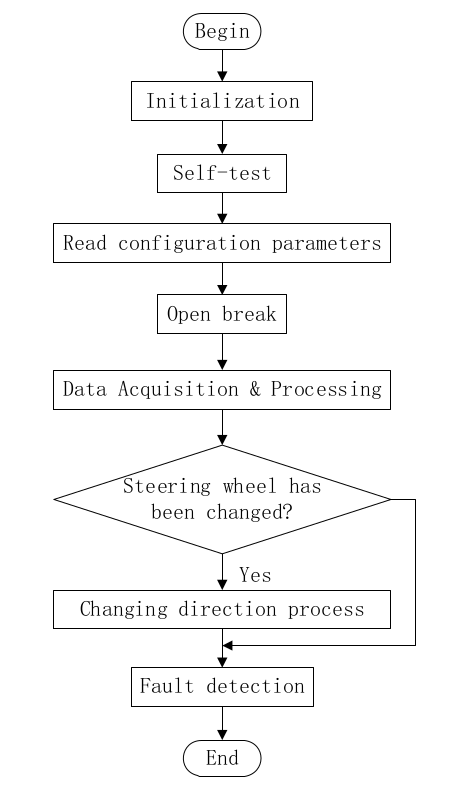
\includegraphics[width=0.5\linewidth]{main_flujo.png}
\end{figure}

\begin{lstlisting}[caption=Extracto de código de \cite{code-2}.,label={ifanidados}]
 if _py_timestamp is not None:
        # Initialize from PyTimestamp, if available.
        self._py_timestamp = _py_timestamp
    elif timestamp is not None:
        # If Timestamp is available, copy its contents.
        self._py_timestamp = timestamp._py_timestamp
    else:
        if is_top and not is_bottom and coordinates is None:
            self._py_timestamp = PyTimestamp(coordinates, is_top, is_bottom)
        elif is_bottom and not is_top and coordinates is None:
            self._py_timestamp = PyTimestamp(coordinates, is_top, is_bottom)
        elif coordinates is not None and not is_bottom and not is_top:
            self._py_timestamp = PyTimestamp(coordinates, is_top, is_bottom)
        else:
            raise ValueError(
                "Timestamp should either have coordinates"
                "or be either Top or Bottom"
             )
\end{lstlisting}


En contraposición a estos trabajos, existen otros \cite{good-desing-agrobot,good-desing-street} que tienen en cuenta algunos principios fundamentales de la IS a la hora de diseñar y destinan esfuerzo en crear software de cierta calidad. Sin embargo, esto no significa que el uso de patrones de diseño esté generalizado.

Por otro lado, existen múltiples trabajos que abordan ``patrones de diseño'',  inspirándose en la manera de documentar que utilizan los autores en \cite{Gamma:1995:DPE:186897}, aplicados a ámbitos particulares. Entre ellos podemos encontrar los siguientes:

\begin{itemize}
\item \cite{enjambre}, se definen patrones de diseño para \gls{enjambresroboticos} en conjunto a un formato de documentación particular. Los patrones se centran en diferentes comportamientos comunes que deben realizar los robots en este tipo de sistemas, como intercambiar información o llevar a cabo cierta interacciones.

\item \cite{patterns_2013}, presenta tres patrones orientados al control autónomo de robots. Parecen estar más cerca de arquitecturas ya que definen el funcionamiento general de ciertos sistemas sin definir módulos y sus interfaces.

\item \cite{stable} donde se describen patrones que ayudan a desarrollar familias de sistemas robóticos estables, definiendo familia de sistemas como ``estable'' a una familia de sistemas modelada, diseñada e implementada de manera que las aplicaciones específicas de dicha familia puedan desarrollarse reutilizando, adaptando y especializando conocimientos, arquitecturas y componentes existentes.

\item \cite{critical} se encuentran patrones de diseño tanto para hardware como software aplicados a sistemas donde la seguridad es crítica debido a su naturaleza. Las aplicaciones de este tipo pueden provocar consecuencias considerables en caso de fallos. La mayoría de los ``patrones'' descriptos se centran en la redundancia y control de resultados. Además de documentarlos, el autor agrega un análisis de impacto en el coste computacional, con el fin de justificar que su aplicación no genera un impacto considerable.

\end{itemize}

Podría pensarse entonces que existen múltiples trabajos que abordan patrones de diseño para sistemas embebidos de control o robóticos, sin embargo, no es exactamente así. En los trabajos mencionados, se utiliza el concepto de patrón de diseño, pero no al nivel de diseño que se trabaja en la IS. Los patrones presentados son \textit{soluciones probadas para ciertos problemas recurrentes}, pero el cambio \textbf{no} aparece involucrado entre esos problemas. Es decir, los autores detallan cómo aplicar una solución a diversos inconvenientes comunes en sus áreas de estudio, pero no incluyen al diseño para el cambio a la hora de su confección. Por ejemplo, un patrón de diseño presentado en \cite{robotArg} es \textit{Patrón de Diseño para el control de un robot diferencial}. Este provee una solución que permite implementar de manera simple un sistema de control especifico. Pero no se pone al diseño para el cambio como una variable a tener en cuenta, la solución no lo considera. Por lo que el resultado de su aplicación no es software preparado para el cambio.

Además, en estos trabajos no se estudian módulos ni interfaces, sino componentes del sistema, algo más parecido a una arquitectura de software. De hecho, se llegan a documentar patrones para hardware, como ocurre con muchos de los patrones definidos en \cite{critical}. En el trabajo \cite{stable} se considera el hecho de reutilizar software, pero los patrones descriptos corresponden a un nivel de abstracción superior al que se busca en esta tesina. Tratan la interacción de diferentes componentes, similar a una arquitectura de software.

De todas formas, es notable como la comunidad de Robótica ha comenzado a discutir sobre la necesidad de aplicar técnicas y principios de IS para construir software robótico mantenible, reusable y modificable \cite{mejoras-1, mejoras-2}. Una prueba del interés son desarrollos como \cite{FernandezMadrigal2003, model,model1,model2,model3}, en los cuales se integran de diferentes maneras, prácticas de la IS en el desarrollo de sistemas embebidos. Por un lado desarrollando \glspl{framework} y arquitecturas orientadas a este tipo de software, como también definiendo metodologías de trabajo. Estos \glspl{framework} no son los únicos orientados a este tipo de sistemas, existen por ejemplo \cite{framework-1, framework-ros}, los cuales son una combinación de sistema operativo y framework. Representan fuertes herramientas para el desarrollo, principalmente, solucionan algunos inconvenientes recurrentes y le quitan responsabilidades al desarrollador resolviendo cuestiones relacionadas con el acceso al hardware, concurrencia, etc., es decir, proveen una capa de abstracción a partir de la cual lo desarrolladores pueden empezar a trabajar. Son ampliamente utilizados en la industria aplicados a grandes sistemas. No así para aplicaciones de menor tamaño, ya que proveen una estructura mayor a la necesaria, complejizando innecesariamente el sistema.

Otra prueba de interés son trabajos como \cite{Shin15fase}, en los cuales se considera agregar formación relacionada a la IS en cursos de robótica y sistemas embebidos. Con igual énfasis en ingeniería de software y robótica, el curso busca enseñar a los estudiantes cómo se aplica la IS a la robótica. En particular, se dan dos lecturas principales que contienen los conceptos de patrones de diseño y arquitectura de software. En la primer lectura se trabaja sobre los patrones \textit{Observer}, \textit{State}, \textit{Strategy} y \textit{Visitor}. El patrón \textit{Observer} se utiliza extensivamente en \gls{ros} para la comunicación. El patrón \textit{State} es útil para implementar el algoritmo de evitación de obstáculos, que consta de varios estados. El patrón \textit{Strategy} permite intercambiar fácilmente diferentes estrategias de planificación de rutas. El patrón \textit{Visitor} es útil para implementar diferentes métodos de predicción y actualización en la localización. En la segunda lectura, se discuten diferencias entre múltiples arquitecturas utilizadas en el campo, tales como CARMEN \cite{carmen}, MOOS \cite{moos}, Microsoft Robotics Studio \cite{microsoft} y \gls{ros}. 

Una de las principales motivaciones es la introducción de la robótica al mercado de consumo masivo fomentando la demanda de reducir los costos del software preservando sus cualidades \cite{Brugali2009}. A medida que los sistemas embebidos incluyen más funciones para nuevos servicios, el software crece gradualmente en tamaño, y los costos y el tiempo de desarrollo también \cite{model2}. En particular, el diseño orientado al cambio, es una de las herramientas claves de la IS para conseguirlo, ya que promueve la reusabilidad del software, haciéndolo aplicable a distintos proyectos y entornos. Esta es una muestra de que la implementación de patrones de diseño es una solución potencialmente útil y deseada.

En línea con este enfoque, en esta tesina se presentaran algunos problemas recurrentes en el dominio de la robótica y se propondrán algunas soluciones de diseño basadas en patrones de diseño con el objetivo de construir software de calidad.

